\section{Čvorovi naredbi}
\label{sec:MyASTStatementNodes}

Naredbe su najkomplikovanije za apstrahovanje zbog njihove raznovrsnosti. Programski jezici često uvode nove sintaksne strukture i naredbe koje nisu do tada viđene u ostalim jezicima. Uprkos svemu tome, ipak je moguće uočiti neke sličnosti sa već postojećim konceptima i svesti ih na isti nivo. Na slici \ref{fig:StatementNodes} se mogu videti tipovi apstraktnih konstrukcija koje će se koristiti da bi se predstavile naredbe.

\begin{figure}[h!]
    \centering
        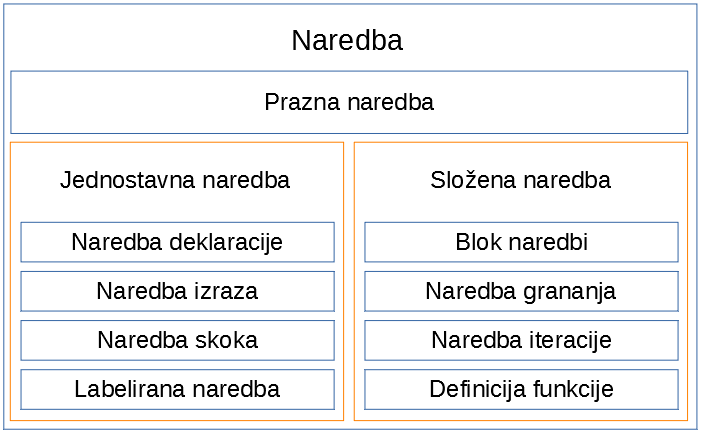
\includegraphics[scale=0.7]{images/statement_nodes.png}
    \caption{Vrste čvorova naredbi.}
    \label{fig:StatementNodes}
\end{figure}
